\documentclass[a4paper,titlepage]{book}     	%base
\usepackage[T1]{fontenc}
\usepackage[utf8]{inputenc}
\usepackage[english]{babel}
\usepackage{geometry} 							%margini
\geometry{a4paper, top=2.5cm, bottom=2.3cm, left=2.3cm, right=2.3cm, heightrounded, bindingoffset=1cm}
\usepackage{verbatim}  							%ambiente commento

\usepackage[nouppercase]{frontespizio}%frontespizio
\usepackage{pdflscape}    						%pagina orizzontale
\usepackage{emptypage}

\usepackage{amsmath, amssymb, mathtools,bm} 					%matematica
\usepackage{siunitx}\sisetup{exponent-product = \cdot}   

\usepackage[english]{varioref}							%vref
\usepackage{hyperref} 							%coll. ipertestuali   ->commentato per usarlo con pdfa
\hypersetup{hidelinks}
%,colorlinks=true,linkcolor=black,citecolor=blue, urlcolor=blue} 							%nascondi riquadri hyp.
\usepackage{booktabs} 							%tabelle
\usepackage{threeparttable}	
\usepackage[labelfont=bf, font=small]{caption} 	%didascalie
\usepackage{import} 							%inkscape



%bibliografia
\usepackage[autostyle]{csquotes} 				
\usepackage[backend=biber, style=numeric-comp, maxnames=1,sorting=none]{biblatex}  %  style=authoryear-comp, style=numeric-comp, sorting=none sorting=nyt,sortlocale=en_GB  maxnames=1,uniquelist=false,
\addbibresource{biblio.bib}

\AtEveryBibitem{%
	\ifentrytype{article}{
		\clearfield{eprint}%
		\clearfield{url}%
	}{}
	\ifentrytype{ARTICLE}{
		\clearfield{eprint}%
		\clearfield{url}%
	}{}
}


\newcommand{\aap}{Astronomy and Astrophysics}
\newcommand{\aapr}{Astronomy and Astrophysics Review}
\newcommand{\aaps}{Astronomy and Astrophysics, Supplement}
\newcommand{\apj}{Astrophysical Journal}
\newcommand{\apjl}{Astrophysical Journal, Letters}
\newcommand{\araa}{Annual Review of Astronomy and Astrophysics}
\newcommand{\bain}{Bulletin Astronomical Institute of the Netherlands}
\newcommand{\mnras}{Monthly Notices of the Royal Astronomical Society}
\newcommand{\nat}{Nature}
\newcommand{\pasa}{Publications of the Astronomical Society of Australia}
\newcommand{\prl}{Physical Review Letters}


%numeri di pagina ai bordi e nomi capitoli fighi
\usepackage{fancyvrb}
\usepackage{fancyhdr}

\pagestyle{fancy}
\renewcommand{\chaptermark}[1]{\markboth{#1}{}}
\renewcommand{\sectionmark}[1]{\markright{\thesection\ #1}}
\fancyhf{}
\fancyhead[LE, RO]{\scshape\thepage}
\fancyhead[LO]{\scshape\small\nouppercase{\rightmark}}
\fancyhead[RE]{\scshape\small\nouppercase{\leftmark}}

%nuovi comandi
\newcommand{\sun}{\ensuremath{_\odot}} 	
\newcommand{\mzams}{M_\textup{ZAMS}}
\newcommand{\zzams}{Z_\textup{ZAMS}} 
\newcommand{\mdot}{\ensuremath{\dot{M}}}
\newcommand{\msun}{\ensuremath{M\sun}}
\newcommand{\zsun}{\ensuremath{Z\sun}}
\newcommand{\yr}{\text{yr}}
\newcommand{\rluno}{\ensuremath{r_\textup{L,1}}}
\newcommand{\rldue}{\ensuremath{r_\textup{L,2}}}


%sommario
\newenvironment{abstract}{\newpage \thispagestyle{empty} \vspace*{3\baselineskip}
	\begin{center}\Large\textbf\abstractname\end{center}
	\begin{quotation}
	}{\end{quotation}\clearpage}

%pdf-a
%\usepackage[a-1b]{pdfx}
%\usepackage[pdfa]{hyperref}
%\hypersetup{hidelinks} 

%%%%%%%%%%%%%%%%%%%%%%%%%%%%%%%%%%%%%%%%%%%%%%%%%%%%%%%%%%%%%%%%%%%
%%%%%%%%%%%%%%%%%%%%%%%%%%%%%%%%%%%%%%%%%%%%%%%%%%%%%%%%%%%%%%%%%%%
\begin{document}
\frontmatter

\begin{frontespizio}
	\Preambolo{\renewcommand{\frontinstitutionfont}{\fontsize{15}{12}\bfseries}}
	\Preambolo{\renewcommand{\frontdivisionfont}{\fontsize{16}{30}\selectfont}}
	\Preambolo{\renewcommand{\frontpretitlefont}{\fontsize{16}{20}\scshape}}
	\Preambolo{\renewcommand{\fronttitlefont}{\fontsize{19}{35}\bfseries}}
	\Preambolo{\renewcommand{\frontnamesfont}{\fontsize{15}{20}\bfseries}}
	\Preambolo{\renewcommand{\frontfixednamesfont}{\fontsize{13}{20}\selectfont}}

	\Istituzione{Università degli studi di Padova}
	\Logo[3cm]{logo}
	\Divisione{\vspace*{1mm}Dipartimento di Fisica e Astronomia ``Galileo Galilei'' }
	\Scuola{Master Degree in Astrophysics and Cosmology}
	\Titoletto{Final dissertation}
	%\Annoaccademico{2019--2020}
	\Piede{Academic Year 2021--2022}
	\Titolo{\vspace*{-15mm} Black hole - Wolf-Rayet binaries as \\ progenitors of binary black holes}
	\NCandidato {Candidate}
	\Candidato {Erika Korb}
	\NRelatore {Supervisor}{}
	\Relatore {Prof. Michela Mapelli}
	\NCorrelatore {Co-supervisor}{}
	\Correlatore {Dr.~Giuliano Iorio}
	\Rientro{2cm}
\end{frontespizio}	

\
\begin{abstract}
	\addcontentsline{toc}{chapter}{Abstract}
I study the formation of binary black hole systems by means of population-synthesis simulations, with the code SEVN (Stellar EVolution for N-body). My main goal is to determine their formation history, with particular attention to mass transfer processes (stellar winds, Roche Lobe overflow, common envelope). I focus my work on the formation channels that include the production of a Wolf-Rayet - black hole binary, finding that this is the most common formation pathway at solar metallicity. I compare my results with the properties of the observed Wolf-Rayet - black hole systems, including the Cyg X-3 binary.

\end{abstract}

\tableofcontents
\addcontentsline{toc}{chapter}{Contents}

%%%%%%%%%%%%%%%%%%%%%%%%%%%%%%%%%%%%%%%%%%%%%%%%%%%%%%%%%%%%%%%%%
\mainmatter

\chapter{Black holes binaries as sources of gravitational waves}
%2-3 pages of overview of GW sources and the problem to understand their formation and have observable candidates in the previous phases, like the X-ray binaries and in particular the WR-BH phase, where the WR maycome from mass transfer interactions. Here I cite the paper apple and oranges of Kalogera 2021 on the tension on the spins
\section{Gravitational waves theory and measurable parameters}
According to the theory of general relativity, an observer in the weak-field limit can detect the gravitational waves as a linear perturbation of the space-time metric. Einstein's theory predicts that the the amplitude of the gravitational wave $h$ is proportional to the second derivative with respect to time of the mass quadrupole moment of the source. Intuitively, a dipolar moment is not sufficient to produce a gravitational wave because the asymmetry in the mass distribution can be re-absorbed just by shifting the origin of the coordinate system. Moreover, requiring a non-zero second derivative with respect to time of the mass quadrupole moment implies that the energy emitted by the system in the form of gravitational waves is extracted from a change in the mass distribution. \cite{MaggioreGW}

\subsubsection{A toy model for circular binaries}\label{subsubsec:toymodel}
A binary system can produce gravitational waves because it has a non-zero quadrupole moment that increases as the binary evolves and shrinks. To get an order-of-magnitude estimate of the measurable quantities it is possible to use the toy model of a circular binary where Newtonian mechanics is dominant and all the orbital energy lost is converted into gravitational wave radiation.  According to the toy model, the binary produces a gravitational wave with amplitude $h$

\begin{equation}\label{eq:h}
	h = \frac{1}{r} \frac{4G\mu\omega_s^2R^2}{c^4}
\end{equation}

where $G$ is the gravitational constant, $c$ the speed of light, $r$ the luminosity distance of the source, $R$ the orbital radius, $\mu=(M_1 + M_2)/(M_1 + M_2)$ the reduced mass and $\omega_s$ the angular frequency. The mass quadrupole moment of a circular binary is symmetric under a rotation of $180^\circ$, implying that every half orbit the phase of the gravitational wave is the same and that the observed frequency is twice the rotational frequency of the source $\nu_{\rm GW} = 2 \nu_s$. \cite{GWreview}

Recalling that the angular frequency $\omega_s=v_s R$ is proportional to the orbital velocity $v_s$ and separation $R$, Eq.\ \ref{eq:h} indicates that the closer the binary, the faster the rotation and the higher the amplitude of the gravitational wave: a close binary system that spirals-in and then merges produces a typical \emph{chirp} signal with amplitude and frequency increasing up to a maximum value, reached at the coalescence. By using Kepler's third law it is possible to describe the variation of the rotational frequency $\nu_s$ and relate it to the \emph{chirp mass} $\mathcal{M}$, defined as

\begin{equation}\label{eq:Mchirp}
	\mathcal{M} = \left(\mu^3 (M_1 + M_2)^2\right)^{1/5} = \frac{(M_1M_2)^{3/5}}{(M_1+M_2)^{1/5}}
\end{equation}

and derivable as

\begin{equation}\label{eq:Mchirp_obs}
	\mathcal{M} = \frac{c^3}{G} \left(\frac{5}{96}~ \pi^{-8/3}~\nu_{\rm GW}^{-11/3}~ \dot{\nu_{\rm GW}}\right)^{3/5}
\end{equation}


Eq.\ \ref{eq:h} also indicates that the stronger signals are the one produced by the heavier binaries, thus favouring the detection of binaries made up by two compact objects, either black holes or neutron stars. The compactness allows the two massive objects to spiral-in in very tight orbits and reach coalescence only when their orbital separation is about the sum of the two Schwarzschild radii

\begin{equation}\label{eq:Rcoalescence}
	R_{\rm coalescence} = \frac{2G}{c^2} (M_1 + M_2)
\end{equation}

i.\ e.\, by using Kepler's third law and the relation $\nu_{\rm GW} = 2 \nu_s$, when the emitted gravitational wave has its maximum frequency

\begin{equation}\label{eq:omegapeak}
	\nu_{\rm GW, max} = \frac{1}{\pi \sqrt{8}}\frac{c^3}{G(M_1+M_2)}
\end{equation}



\subsection{Typical observable values for merging compact object binaries }
Binaries with different properties (component masses and spins, orbital separation,  $\dots$) generate different waveforms for the spiral-in, coalescence and ringdown phase. Thus, the detection pipeline of the gravitational wave interferometers of the LIGO Scientific, Virgo and KAGRA Collaboration identifies and characterizes the properties of the binaries by match-filtering the recorded signal with gravitational waveform templates generated with numerical relativity. Nevertheless, the toy model explained in Sec.\ \vref{subsubsec:toymodel} can still be used to get an order-of-magnitude estimate of the main binary properties.

The peak of the chirp signal of a merging binary provides all the necessary informations to estimate the masses, final orbital separation and luminosity distance of the source. According to Eq.\ \ref{eq:omegapeak}, the peak frequency of the gravitational wave is inversely proportional to the total mass of the system: since higher frequencies correspond to stronger wave amplitudes (Eq.\ \ref{eq:h}), in principle is easier to detect a neutron star binary rather than a black holes binary.

During the latest observing run O3, ended in March 2020, the gravitational wave interferometers of the LIGO Scientific, Virgo and KAGRA Collaboration had a peak sensitivity of $h \sim 10^{-23}~ \rm Hz^{-1/2} $ at $\nu_{\rm GW} \sim 100 \rm Hz$, as reported in Fig.\ \ref{fig:sensitivity}



\begin{figure}
	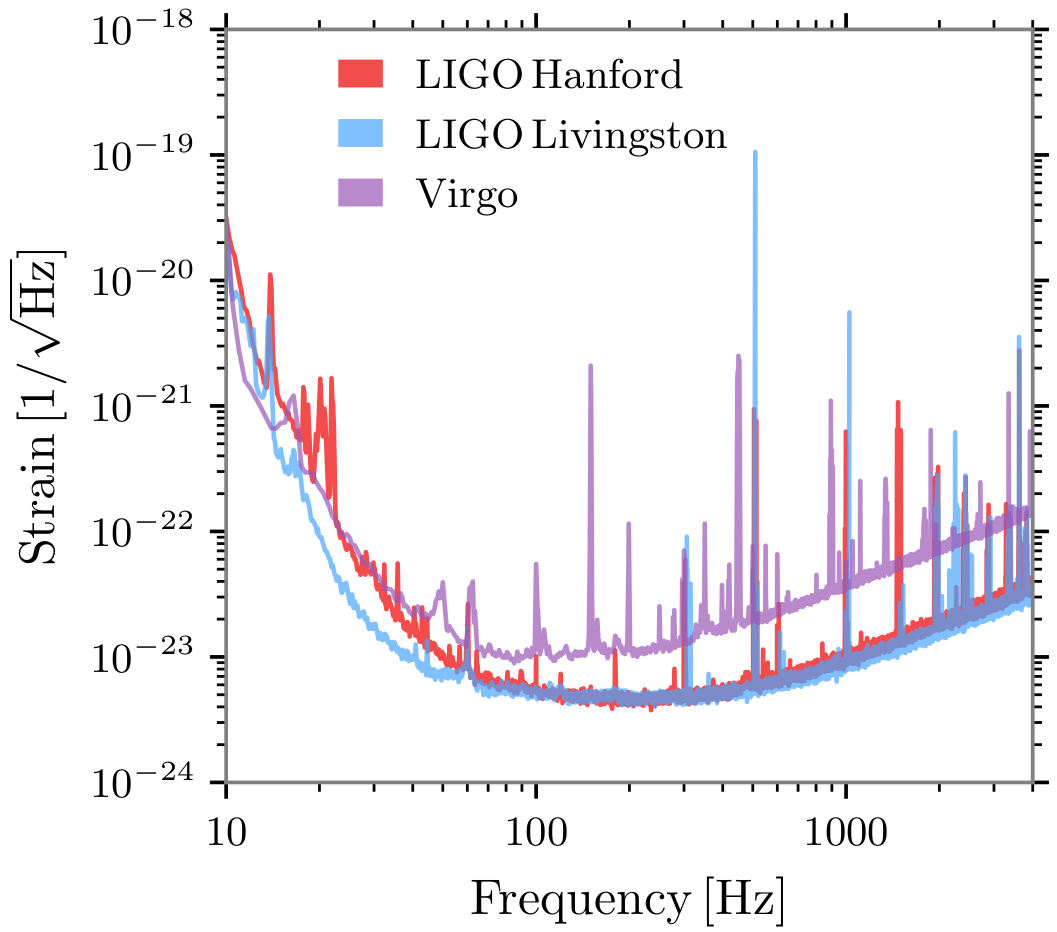
\includegraphics[width=\textwidth]{./images/sensitivity.png}
	\caption{Sensitivity curves of the LIGO and Virgo interferometers during the third observing run. \cite{GWTC-3}}\label{fig:sensitivity}
\end{figure}


The only sources of gravitational waves detected so far are the binaries of compact objects i.e. the binaries made up by two black holes, two neutron stars or a black hole and a neutron star. The gravitational waves have been observed either indirectly or directly: in the first case it was possible to measure the decay of the orbital period of the Hulse-Taylor pulsar over 30 years \cite{HTpulsar2005GWdecay}; in the second case the interferometers of the LIGO Scientific, Virgo and KAGRA Collaboration measured the perturbation of the metric on Earth as caused by $\sim 90$ merging compact object binaries \cite{GWTC-3}. 



 that can be generated when a compact source has a quadrupole moment that changes with respect to time. In particular, the amplitude of the wave $h$ is proportional to the second derivative with respect to time of the quadrupole moment of the source, meaning that the stronger perturbations are produced by very compact, heavy and rapidly rotating objects. \\

A typical source of gravitational waves is a tight binary of compact objects (black holes or neutron stars): the masses are orbiting and are distributed with a quadrupolar moment with respect to the center of mass. Moreover, the symmetry of the system implies that a distant observer sees that same mass distribution with respect to the center of mass (i.e. the same quadrupole moment) every half orbit

the mass distribution with respect to the center of mass as seenfrom a distant observed, therefore the quadrupole moment changes with twice the rotational frequency. 

 circular and tight binary system composed by two compact objects  emits a gravitational wave signal with amplitude $h$ given by: proportional to the second derivative with respect to time of the quadrupole moment of the source: the heavier the masses involved and the faster they rotate, the stronger will be the space-time perturbation. For a circular binary


\section{GWTC-3 and its implication for the progenitor evolution}
In September 2015, the detection of the first gravitational wave GW150914 not only confirmed the existence of binary systems made of two stellar black holes but also demonstrated that such systems are capable of merging via emission of gravitational waves within a Hubble time $H_0$ \cite{Abbott2016firstGW}. In March 2020, the LIGO Scientific, Virgo and KAGRA Collaboration ended the third observing run and, by November 2021, produced the third Gravitational-Wave Transient Catalog (GWTC-3), revealing a total of $\sim 80$ merging binary black holes discovered with the gravitational waves detectors \cite{GWTC-3}.\\







The shape of the gravitational wave signal of a merging binary depends on many astrohphysical parameters: some of them are dominant in the inspiral



; it is possible to characterize the binary properties using the numerical relativity techniques to generate a set of templates for the gravitational waveform for a given set of parameters and then obtaining them by fitting th

 like the luminosity distance, 








The sources added in the GWTC-3 catalogue shed new light on the mass and spin distribution of the merging binary black holes \cite{GWTC-3_interpretation}. 




\cite{Abbot2021spectrumGW,HMXBH_spins2021} analyzed the remnant properties of the GWTC-2 catalogue (\cite{GWTC-2}) and concluded that such systems could both evolve from isolated binaries in the galactic field and from dynamically active environments, such as young star clusters. The observations revealed merging BBHs with very different combinations of masses and spins, providing a precious sample to test and perfectionate the aformentioned models. In fact, in the first scenario, we expect that the evolution is dominated by binary processes like the Common Envelope (CE) and the Roche Lobe Overflow (RLO), that favour the sharing of mass and angular momentum between the two components and the production of remnants with aligned spins (\cite{Kalogera2000_spinaligned}) and similar masses, up to $\sim 50~\msun$ (\cite{Giacobbo2018spectrum}). In the second scenario we expect that hierarchical mergers and binary exchanges allow the formation of BHs in the pair-instability gap ($\sim 60-120~\msun$), with mass ratios $q=M_2/M_1$ far from unity (\cite{Rastello2021_dynamics}) and misaligned spins (\cite{Rodriguez2016_BHspins}).

From an observational point of view, BBHs progenitors can be searched in binary systems that already contain a stellar BH. Nevertheless, BHs in quiescent systems are very difficult to observe with radial velocity (\cite{BHradialvelocity}) and astrometric measurements (\cite{GaiaDR2microlensing}) and hopefully the new Gaia Data Releases will shade more light on them. On the contrary, BHs can be visible in the X-ray band if they are accreting mass from a companion star. These systems are called Black Hole X-Ray Binaries (BH-XRBs) and, according to \cite{HMXBH_spins2021}, their progenitors share the same mass distribution of the progenitors of the primary BHs in the GWTC-2 catalogue (although the GW-BBHs progenitors exhibit slower spins, which leaves the debate open).



In this paper we will focus on the BH-XRBs systems made up by a Wolf-Rayet (WR) and a BH (hereafter, WR-BH systems) and we will try to constrain the conditions under which they could be progenitors of GW-BBHs systems in the isolated binary evolution scenario. We expect that these are very good candidates to form a GW-BBH, given that at solar metallicity $Z=\zsun=0.02$ the WRs are formed from stars with initial mass $\mzams \gtrsim 30~\msun$ (\cite{Limongi2010_preSNevo}), have strong line-driven winds and high mass loss rates $\mdot \sim 10^{-4}-10^{-5}~\msun$/yr (\cite{G&H_WRmassloss}). This means that WR stars are more likely to form a secondary BH in the neutrino-driven SuperNova (SN) scenario (threshold at $\mzams \gtrsim 25~\msun$ for BH formation, \cite{Sukhbold2016_stellarevo}), and to produce a bright accretion disk around the primary BH ($L_\textup{X} \gtrsim 10^{36}$~erg/s, \cite{Tutukov2013_WRBHreview}).





\chapter{Theory and observations of Wolf-Rayet - black hole systems}
\section{Single stellar evolution to form a WR}
Little recap of single stellar evolution on what is and how evolves a WR, underlying e.g. the typical progenitor masses and the importance of the stellar winds.\\


PLOT: SSE of 30 and 40 Msun with Z=0.015 and 0.02 to show influence of mass and stellar winds.

\section{Mass transfer in binary systems}
Short overview of the main binary processes, with particular attention to the wind accretion, Roche lobe overflow and common envelope


\section{Observed candidates of Wolf-Rayet - black hole systems}
The core is the paragraph I already wrote for the Computational Astrophysics exam (a table with the observed properties and short explanations on the uncertainties of the measurments). Brief review of the literature on possible evolutions of the systems as GW mergers.\\



%%%%%%%%%%%%%%%%%%%%%%%%%%
%%%%%%%%%%%%%%%%%%%%%%%%%
\begin{figure*}
	\begin{threeparttable}
		\begin{tabular}{llccccc}
			\toprule
			Host galaxy & Name & BH mass [$\msun$] & WR mass [$\msun$] & Period [h] & $t_\textup{GW}$ [Gyr]  &Z [$\zsun$] \\
			\midrule
			IC 10 & IC10 X-1 & 23-33\tnote{a} & 35\tnote{b} & 34.9\tnote{a} & 3.5  & 0.22 \\
			NGC 300 & NGC300 X-1 & 13-21\tnote{d} & 26\tnote{c} & 32.8\tnote{d} & 2.9  & 0.19 \\
			M101 & M101 ULX-1 & 20-30 & 19& 196.8 & 348 & 0.17 \\
			Milky Way & Cyg X-3 & 3 & 7 &4.8 & 0.017 & 0.31 \\
			NGC 4490 & CXOU J123030.3+413853 & - & - & 6.4 & 0.038  & 0.23 \\
			NGC 253 & CXOU J004732.0-251722.1 & - & - & 14.5 & 0.33  & 0.24 \\
			Circinus & CG X-1 & - & - & 7.2 & 0.051  & 0.10 \\	
			\bottomrule 	
		\end{tabular}
		\begin{tablenotes}[para]
			\item[a]\cite{IC10X-1_Silverman2008} 
			\item[b]\cite{IC10X-1_Clark2004_WRmass}
			\item[c]\cite{NGC300X-1_Crowther2010} 
			\item[d]\cite{NGC300X-1_Binder2021_BHpreciso}
		\end{tablenotes}
		\centering
		\captionof{table}{Properties of the seven WR-BH candidates. The table is inspired by \cite{observations}. $t_\textup{GW}$ is an order-of-magnitude estimate calculated assuming $M_{1,\rm BH} = M_{2,\rm BH} = 10~\msun$, given the uncertainties in the mass determination discussed in Section . The other parameters are extracted from the above referenced papers and from \cite{M101ULX-1_Liu2013} (M101 ULX-1), \cite{Cyg-X3_Zd2013} (Cyg X-3), \cite{NGC4490cand_Esposito2013c} (CXOU J123030.3+413853), \cite{NGC253cand_Maccarone2014} (CXOU J004732.0-251722.1), \cite{observations} (CG-X1), \cite{observationsZSFR_Mapelli2010a} (Z).} \label{tab:observations}
	\end{threeparttable}
\end{figure*}
%%%%%%%%%%%%%%%%%%%%%%%%%
%%%%%%%%%%%%%%%%%%%%%%%%%

\section{Cyg X-3}
Review of Koljonen+2017 and discussion on why values of Zdiarski+2013 are not reliable and we don't use them. Also describe it is in the MW and how we determined its metallicity and distance.
\subsection{Properties}

\subsubsection{Observations and identifications}
Cyg X-3 lies in the galactic plane therefore no optical/UV counterpart has been detected yet due to interstellar absorption (\cite{CygX-3_Koljonen2017}). Thus we know that the companion is a WR only by observing its IR spectrum. Using IR and X-ray emission lines, the companion is a low-mass BH or a NS.

\subsubsection{DIstance and metallicity}
\textbf{McCollough2016} on the galactic plane ($l=79.84^\circ, b=+0.70^\circ$). Distance 7.4 $\pm$ 1.1 kpc or, but less, probable, 10.2 $\pm$ 1.2 kpc. Distance estimated by looking at the "little friend" of Cyg X-3 i.e. a nearby Bok globule that was observed in X-ray by Chandra and then followed up with Submillimetric observations. This Bok globule is a 2-24 \msun gas+dust cloud confined in a 0.2 pc that scatters towards us the X-ray radiation produced in the nearby X-ray binary. Assuming that the velocity shift of the CO line is due only to the galactic rotation, the authors could use a tool for modeling the motion on the galactic disk and reconstructed a distance of 7.4 or 10.2 kpc (two values because of possible errors in the tool evaluation but the first is more probable).\\

We expect that Cyg X-3 was born in the star-forming region associated to the Bok globule and then the SN kick that formed the BH expelled the system from the Bok globule. Given that the binary is $\sim 1$ kpc away from the Bok globule and the lifetime of the WR, therefore the time elapsed from the SN, is $\sim 1-5 \times 10^6$ years, the authors estimate a SN kick of $\sim 190-980$ km/s, in agreement with some upper and lower independent constraints.\\

To model its metallicity we use the metallicty gradient of the MW that was obtained by \textbf{Lemasle2018} using Gaia data of metallicity and distance of 25 Cepheids. They found \[[Fe/H]=-0.0447*d_{\rm Galacto}(kpc) + 0.3522\]. By tringulation, the galactocentric distance of Cyg X-3 is $d_{\rm Galacto} = 9.85$ kpc ($l=79.84^\circ$, heliocentric distance = 7.94 kpc from Lemasle 2018 and relative distance of Cyg X-3 = 7.4 kpc from the measurements on the BOk globule carried out by McCollough 2016). We therefore obtain \[[Fe/H] = -0.088095\] and, assuming that the metallicity distribution of the Sun is universal, we can convert such value to the metal mass fraction using \[[Fe/H] = log(Z/X)_* - log(Z/X)_\odot\] i.e. we obtain \[Z_* = 0.91567 \zsun\]. If we assume \zsun=0.02 we get $Z_*=0.0183$ but if we assume \zsun=0.01524 we get $Z_*=0.01395$.

\subsection{Period}
\subsubsection{Singh 2002} 4.8 hours. We take a larger range i.e. 4.5 - 5.1 hours, that combined with the possible mass ranges for WR and BH results in a semimajor of $a \sim 3-4 $ Rsun


\subsection{Mass ranges}
\subsubsection{Koljonen \& Maccarone 2017} I used WR = 8 - 14 \msun, BH = 3. - 10 \msun \\

They derived: ?? \\

Model: X-ray emission from compact object ionizes the stellar wind of the WR and causes the emission lines visible in the NIR (1-2.4 $\mu$m). They use a non-LTE model for the atmosphere of the WR to reproduce the continuum + emission lines in the NIR. \\

Semimajor axis according to my model: Minimum possible a=3.052 Rsun with P=4.5 hours and Mtot = 8+3=11 \msun .  Maximum possible a=4.303 Rsun with P=5.1 hours and Mtot = 14+10=24 \msun 


\subsubsection{Zdziarski 2013} \cite{Cyg-X3_Zd2013} I used WR = 7.5 - 14.2 \msun, BH = 3 - 4.5 \msun \\

THey derived:WR = 7.5 - 14.2 \msun, Compact object = 1.3 - 4.5 \msun and then Belczynski 2012 assumed as MminBH = 2 \msun\\
\\

\subsubsection{Procedure}
Vogliono risolvere un sistema a due variabili \mdot e MWR dove le due equazioni sono eq. 3 e eq 6 nel paper, che, combinate con altri dati osservativi e combinazioni, diventano le equazioni 7 e 8.

La prima descrive il rallentamento della binaria a causa del momento angolare trasportato via dal vento che lascia il sistema. Tale equazione lega Mdot, MWR+MCO, Pdot/P e di essa conosciamo $Pdot/P = 1.03+- 0.02 x 10^{-6} ~ \rm yr^{-1}$ da Kitamoto (comunicazione privata) e possiamo legare MCO alla massa della WR attraverso il mass ratio della binaria q che altro non è che il rapporto tra i due picchi delle due curve di rotazione

\[q = Mcompact/MWR = KWR / Kcompact \sim 0.23\] 

Problema: Ko17 evidenziano che Zd13 hanno usato i dati di Hanson2000 che aveva usato come tracciante per il moto orbitale la linea di assorbimento HeI 2p-2s e che purtroppo è molto probabile che questa linea NON sia un tracciante per il moto orbitale bensì per il campo di velocità del vento della WR. Inoltre, lo spettro usato era stato preso nel 1999 durante un outburst, quando era presente anche una doppia linea di emissione He I 2p-2s a compilcare il tutto. 




Semimajor axis according to my model: Minimum possible a=3.005 Rsun with P=4.5 hours and Mtot = 7.5+3=10.5 \msun .  Maximum possible a=3.96 Rsun with P=5.1 hours and Mtot = 14.2+4.5=18.7 \msun 


\chapter{Models and simulations with SEVN2}
\section{The SEVN2 population-synthesis code}
Interpolates PARSEC tables, describe winds, criteria for identifying a WR, explain how, explain details of mass transfer, explain assumption on the pessimistic case, explain the three kick models, explain the three CCSN models (use histograms)\\
PLOT: histogram with compact remnants with different SN models\\
(PLOT: histogram with compact remnants with different kick models )

\section{Initial conditions for simulations}
Describe the distributions of masses, periods, eccentricities from which I derived the 1 million simulations. Scheme with the parameter space explored

\chapter{Results}
\section{> 90 \% GW-BBH undergo WR-BH configuration}
4 tabelle per i 4 modelli di kick che mostrano che nonostante si varino CCSN e metallicità è incontrovertibile che la WR-BH sia una configurazione obbligata.

\section{Fiducial model}
In dettaglio mostrare hist2d di a vs m1+m2 per progenitori, inizio WR-BH, remnants, m1+m2 vs tgw, m1 vs m2 progenitor, m1 vs m2 remnant.\\
In dettaglio analizzare evoluzione di Cyg X-3 con i trasferimenti di massa e le proprietà di osservabilità tipo il RL filling e la divisione in due/tre famiglie. Grafici: M1 VS M2, RL1fill vs RL2fill, RL1fill vs M1 per discutere il wind-fed, grafico periodo vs tempo in WR-BH per discutere tempo osservabilità, evoluzione di una singola binaria rappresentativa per tipo di mass transfer (RLO+RLO+CE, RLO +CE e CE+CE)

\section{Role of metallicity}
Comparare con stesso kick unified + 265 + CCSN = compact ma scegliendo Z=0.02 e discutere il diverso tempo evolutivo, canali e durata mass transfer e proprietà.
Mostrare gli hist2d per a vs m1+m2 per progenitor e remnant e mostrare che sono gli stessi.\\
Poi usare come prima tre binarie rappresentative per i 3 tipi di mass transfer di Cyg X-3 e discutere le differenze rispeto a Z=0.15. Mostrare anche le differenze nei grafici M1 VS M2, RL1fill vs RL2fill.


\section{Role of the kicks}
Mostrare per Z=0.015 + CCSN= compact che diversi kicks cambiano principalmente il semiasse finale, scatterando molto di più i risultati delle GW-BBH ma lasciando quasi inalterati i candidati Cyg X-3 e la loro evoluzione. Mostrare i 4+4 grafici di a vs m1+m2 remnant e di m1vsm2 di Cyg X-3.

\section{Role of CCSN model}
Comparare prima con il kick fiducial unified+265 e Z=0.015 i tre modelli di CCSN e mostrare per ciascuno 2 grafici: M1 VS M2 per Cyg X-3 e a vs m1+m2 dei remnants. Ricordando le differeze iniziali nei modelli, spiegare le differenze.


\section{Probing the parameter space}
Mostrare a vs m1+m2 remnant e m1vsm2 Cyg X-3 a set di 3 CCSN variando i tre kick prima con Z=0.015 e poi con Z=0.02. Discutere come l'evoluzione di Cyg X-3 rimanga molto simile ma hobbs pure + rapid/delayed scatteri moltissimo le proprietà dei remnant





\section{Compare with Belczynski+2013}
??? Ha senso??




\chapter{Conclusion}
\begin{itemize}
	\item WR-BH as mandatory intermediate configuration needed to form GW-BBH at solar metallicity. Implication for spins (?)
	\item Well-defined properties for Cyg X-3 systems (say which), less defined for GW-BBH but quite well-constrained.
	\item At least a CE is needed + another CE or a stable RLO. Optional a third stable RLO for Cyg X-3 like systems. To be investigated if it is true also for GW-BBH but we think this may be representative for GW-BBH in the region of Cyg X-3
	\item CCSN introduces the most uncertainties in the masses of the remnants, thus selecting the evolutionary paths (e.g. the delayed almost completely removes the stable mass transfer channels)
	\item The kicks most favour the semimajor and when combined with rapid/delayed spread a lot the results
	\item Metallicity changes the stellar evolution and also spreads the results, even though a little less. Most importantly, it may transform the second mass transfer from RLO stable + CE into one single CE after a long RLO, all because the donor MS is able to expand/contract differently therefore R>RL long enough to become unstable before re-entering the RLO
\end{itemize}






\chapter{Annotazioni/Bozza}
With the fiducial model i.e. Z=0.015, SN=compactness, kick=unified, sigma = 265
\begin{itemize}
	\item Probability to form a WR/BH(cyg x-3 like) system in principle out of all binaries
	\item Probability to form a GW-BBH WR/BH(cyg x-3 like) system in principle out of all binaries
	\item Probability a WR-BH(cyg x-3 like) system has 2RLO/RLO+CE/2CE
	\item Probability it is visible in the WR-BH(cyg x-3 like) configuration?
	\item Time from system born, time from WRBH born, time to BHBH, time to merge all as a function of observed period and total mass
	\item probability it is observed as RL filling/wind fed system as function of semimajor
	\item evolutionary pathaway of WRBH (cyg x-3)
\end{itemize}


\subsection{Parameter space to explore}
OPtimistic o pessimistic scenario for RLO \\
Z= 0.02 and Z=0.015\\
SN = rapid, delayed, compact \\
Kicks = hobbs pure + sigma = 70 (Atri 2019, from median of 107 km/s) \\
Kicks = hobbs pure + sigma = 265 \\
+ fiducial \\
+ Belczynski


\subsection{Compare with Belczynski}
Evolve with Z=0.02, SN=rapid, kick=sigma 265 + fallback as Fryer.


Belczynski considered Z=0.02 and sigma=265 always and always obtained a BBH. He varied different parameters though:
\begin{itemize}
	\item rapid + hobbs + fallback = 14.2 WR + 4.5 BH --> 7.4 BH + 4.5 BH
	\item rapid + hobbs + fallback = 14.2 WR + 4.5 BH --> 8 BH + 4.5 BH (\textbf{NugisLamers2000 winds})
	\item rapid + hobbs pure = 14.2 WR + 4.5 BH --> 7.4 BH + 4.5 BH
	\item delayed + hobbs + fallback = 14.2 WR + 4.5 BH --> 3.9 BH + 4.5 BH
\end{itemize}

Cioè con il rapid model, a prescindere dal kick model (=con o senza fallback) ottiene sempre che una WR di 14.2 iniziali diventa un BH di 7.4-8 Msun. Invece con il delayed (e il fallback) il BH è molto più leggero.\\

In ogni caso predicono che il sistema starà in configurazione WR-BH per 0.64 Myr

\subsection{Notes on how SEVN works/how to interpret things/where to focus}
Taglio della tesi: 
\begin{itemize}
	\item Primo aspetto/paper: per diventare GW-BBH a metallicità locale è NECESSARIO passare per la fase di WR-BH. Ammesso e non concesso (forte assunzione) che i GW-BBH osservati attualmente provengano da isolated channel a questa metallicità, ciò significa che gli spin devono essere gli stessi e questo sarebbe un grosso problema, visto che attualmente Vicky \& Kalogera in apple e oranges hanno sottolineato che non è assolutamente la stessa cosa...
	\item Secondo aspetto/paper: cyg x-3 evolve così o colà a seconda del parameter space ma sembra avere proprietà iniziali/finali molto ben definite negli hist2D e ciò rende i risultati abbastanza well-constrained
	\item Per rendere questo risultato un po' più solido bisognerebbe anche esplorare le BH-NS, tutte le WR-BH che non sono cyg x-3, a metallicità più basse
\end{itemize}

Cosa non è chiaro/è da testare

 
\begin{itemize}
	\item Kick = Unified + sigma = 70 km/s non ha senso perché unified è stato calibrato per riprodurre le osservazioni a partire dalla maxwelliana di hobbs. Pertanto è stato pensato per estrarre il kick da una maxwelliana di 265 km/s e poi diminuirne la magnitudine in base a ejecta e massa del remnant. Se parto già con una sigma di 70 sto già estraendo dei kick bassi, non posso diminuirli ancora di più...
	\item Il fatto che con hobbs puro io abbia un sacco di merging BBH ad alti semiassi posso provare a spiegarlo guardando all'eccentricità delle binarie, magari c'entra quanto vicine al periastro passano oppure no
	\item Overcontact binaries da testare perché passano quasi tutte per di là.Inoltre Giuliano spiega: questione overcontact binary: conosco bene questi casi e sono proprio alla base dell’ultima “importante” modifica di SEVN. 
	Precedentemente questi casi andavano tutti a finire in merger o CE, ma ci siamo resi conto che in BSE/MOBSE questo check è disabilitato mentre c’è un RLO. Ora è cosi anche in SEVN. 
	Ho già controllato che questi casi soprattutto durante un HG sono presenti anche in BSE/MOBSE. 
	
	Quindi in sostanza ogni volta che il Raggio>RL e quindi c’è un RLO consideriamo per la stella  un raggio effettivo pari a quello del RL per tutti i vari processi (venti,tides) mentre il Raggio della stella è usato 
	solo per stimare il rate di mass transfer usando l’equazione 58 in Hurley02.
	
	Se questo sia il modo migliore per gestire il mass transfer non saprei, probabilmente no, ma si inserisce nel discorso piu ampio di andare oltre le prescriptions di Hurley. 
	Abbiamo gia visto che lasciare che questi oggetti mergono in realtà è un assunzione che non funziona soprattuto considerando i merge rate delle neutron stars. 
	
	Per fare un discorso pratico e concreto quello che ottieni in SEVN è consistente con Hurley e BSE/MOBSE ed è solo una conseguenza del modello di RLO adottato. 
	Alla fine non ha nemmeno troppo senso avere plot in cui mostri il raggio durante il RLO perché per SEVN in questi casi il raggio effettivo della stella è pari a RL. 
	\item la SN compact è descritta come nel paper della mapelli https://arxiv.org/pdf/2005.03055.pdf dove il grafico in basso è stato fittato con due distribuzioni. Se nel file .sh il parametro -1 è settato, allora la treshold zeta2.5 non è 0.3 come nel paper della mapelli ma viene estrapolata randomicamente da quelle distribuzioni (o una roba del genere). La SN= compactness è MOLTO biasata nel creare BH invece che NS
	\item per la SSE delle pure He posso confrontare la stessa stella se tipo mi faccio printare anche la colonna "zams" che mi dice qual è la traccia che sta usando per l'interpolazione (a seconda della tabella usata)
	\item Capire nel dettaglio le differenze tra Z=0.02 e Z=0.015
	\item Focus sul final fate dopo la WR-BH per un confronto con Belczynski
	\item controllare le incertezze sulle masse di KO17!!! Specialmente la metallicità usata per la M WR dalla relazione M-L
	\item Pessimistic/optimistic case riguarda la possibilità che una stella in HG possa entrare ed eventualmente sopravvivere ad un CE (optimistic) oppure si fonda direttamente con la compagna nell'ipotesi di assenza di un core ben definito (pessimistic)
\end{itemize}

They predict:\\
\begin{itemize}
	\item WR progenitor of 50 Msun produces WR of 14.2 Msun with R=1.2 Rsun and Rlobe = 1.8 in a=3.8 Rsun orbit with a BH of 4.5 Msn as companion
	\item mass loss rates for the WR taken from Hurley 2000 + Hamann \& Koesterke 1998 (theoretical)
	\[\dot{M} = 10^{-13}(L/L_\odot)^{1.5} \msun \yr^{-1}\]
	\item WR lives for 0.64 Myr and becomes a 8.2 Msun WR with CO core of 6.2 Msun and orbit expanded to a=5.6 Rsun. 
	\item rapid core collapse for the WR leads to fallback=1 but with the 10\% of the gravitational mass lost due to neutrinos we obtain a secondary BH of 7.4 Msun with NO NATAL KICK (because the fallback is maximum therefore it is fully damped), slightly wider orbit of a=6 Rsun and e=0.07.
	\item the final BHBH of 7.4 Msun + 4.5 Msun has a chirp mass of 5.0 Msun and will merge in 500 Myr.
\end{itemize}

\textbf{Different wind}:\\
\begin{itemize}
	\item Use wind taken from Nugis \& Lamers 2000 as done in Zdziarski i.e. by selecting the ones for WR stars with the desired masses (empirical based on 64 WR in the MW. In particular in the mass range I am interested, out of the 34 observed WR, 19 were mostly in a binary system)
	\[\dot{M} = 1.9\times10^{-5}(M_{WR}/14.7\msun)^{2.93} \msun \yr^{-1}\]
	\item Slight increase in the BH formed after the WR (8 Msun instead of the previous 7.4 Msun. Probably because they are lower than the theoretical ones so they retain more mass i.e. they form a heavier BH in the end). 
	\item No other appreciable changes
\end{itemize}

\textbf{Different kick}:
\begin{itemize}
	\item if no fallback the probabilty to form a merging BHBH system reduces from 100\% sure to only 68\% because some systems are disrupted by the larger kicks
\end{itemize}


\textbf{Different SN}:
\begin{itemize}
	\item delayed model forms a lighter BH (3.9 Msun instead of the 7.4 Msun) because the delayed explosion allows more mass to escape and not to accrete back. This also lowers the formation efficiency to 50\% 
\end{itemize}



\section{Compactness model implemented in SEVN}
As explained in Mapelli+2020 \cite{mapelli2020_compactness}, the compactness model in SEVN uses the final CO mass to interpolate the compatness parameter

\begin{equation}
	\xi_{2.5} = 0.55 -1.1 \left(\frac{1 \msun}{m_{\rm CO}}\right)
\end{equation}

where the above formula is derived with fits to FRANEC data.\\

Patton and Sukhbold 2020 \cite{COcollapse}, in the bottom figure of Fig. 3, provide the probability that a star with a given compactness parameter undergoes an explosion or implosion. We fitted to that data a probability distribution and use it to randomly decide whether out star with that compactness will explode, forming a NS, or will implode, forming a BH.\\

After the compact remnant is formed, 



\section{Pipeline}
\begin{itemize}
	\item Su demoblack result.py, read.py e WRBH.py per generare i file WRBH, BHBH, BHNS, result.txt e le cartelle dataframes e copied. Il tutto viene salvato in una cartella che identifica la simulazione e si chiama tipo 1mln\_Z015\_com\_unified265
	\item Quest'analisi include nei file WRBH, BHBH e BHNS tutti i corrispondenti candidati usando come criterio di classificazione unicamente la PhaseBSE e NON la massa
	\item La cartella tipo 1mln\_Z015\_com\_unified265 viene copiata sul pc
	\item Si fa debugging per estrarre correttamente i BH, cioè scegliendo se considerare come "veri" BH anche i BH con massa < 3 che si originano dalla PPISN. Per fare ciò si fanno andare gli script result2.py, read2.py e WRBH2.py scegliendo, a seconda, l'opzione desiderata per il debugging: debug= 'ppisn' sceglie come massa minima per i BH in Cyg X-3 quella pari a ?? in base a ?? mentre l'opzione debug='real' seleziona come BHBH e BHNS solo i sistemi dove il BH sia un oggetto compatto con massa > 3
\end{itemize}





\section{Results Cyg X-3}
Present results with different parameters (SN model and metallicity) and show how they impact on the evolution in general. Underline the main evolutionary paths (RLO/CE) and progenitors and remnant properties (like the computational exam)

Then show detailed evolution for Cyg X-3 only, showing differences with Belczynski 2013.





\printbibliography[heading=bibintoc]
\end{document}


